\documentclass[11pt,a4paper]{report}
\usepackage[utf8]{inputenc}
\usepackage[english]{babel}
\usepackage{amsmath}
\usepackage{amsfonts}
\usepackage{amssymb}
\usepackage{graphicx}
\usepackage{listings}
\usepackage{hyperref}
\usepackage[hmargin = 3cm, vmargin = 3cm]{geometry}

\author{Baptiste \textsc{Rouger} \and Nicolas \textsc{Senecaut} \and Nympha Elisa \textsc{Sia}}


\title{Final Exam : Computational Biology}


\begin{document}
\maketitle

\section*{Question 1}

We build the model with 3 variables : N (the density of cell in CFU), E (the concentration of the E protein) and A (the concentration of AHL).\\

\noindent We also have 7 parameters, defined here for pH 7 : \\
\begin{center}
\begin{tabular}{|c|c|c|c|c|c|c|}
\hline
k & N$_m$ & d & k$_E$ & d$_E$ & $\nu_A$ & d$_A$ \\
\hline
$0.97$ & $1.24 \cdot 10^9$ & $4 \cdot 10^{-3}$ & $5$ & $2$ & $4.8\cdot 10^{-7}$ & $0.639$ \\
\hline
\end{tabular}
\end{center}
~\\
The parameter vector will be added in the following questions by the quantity of inducer, the $\theta$ and $\eta$ values.\\

Our model is written in you\_ode.m, such as
\begin{lstlisting}[language=MatLab]
  function xdot= you_ode(t,x,p)

    %x_names= {'N','E','A'}; -> x(1) is N, x(2) is E, x(3) is A
    %p_names= {'k','Nm','d','ke','de','va','da'}; -> p(1) is k,
                                                  % p(2) is Nm, etc
    xdot= zeros(size(x));

    xdot(1) = p(1)*x(1) * (1-x(1)/p(2)) - (p(3)*x(2)*x(1));
    xdot(2) = p(4)*x(3) - p(5)*x(2);
    xdot(3) = p(6)*x(1) - p(7)*x(3);
  end
\end{lstlisting}

\begin{figure}[!ht]
  \begin{center}
    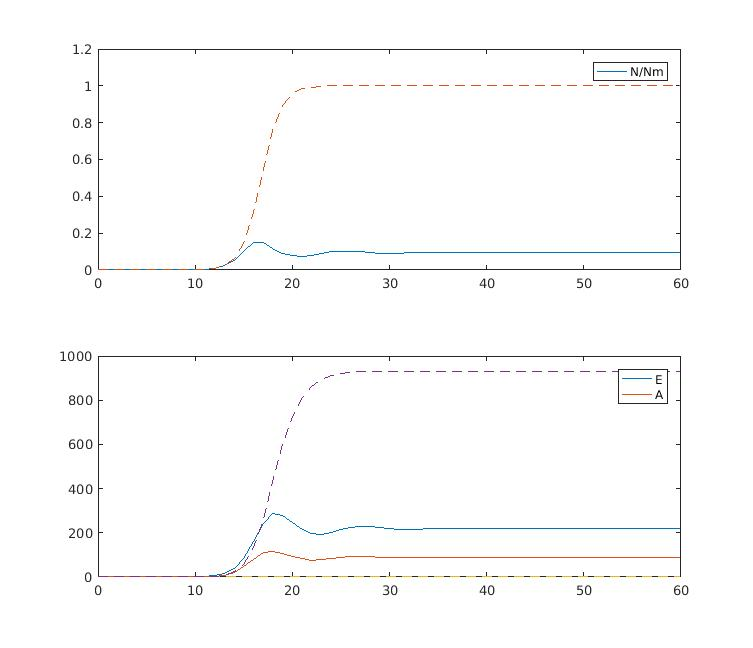
\includegraphics[width=0.7\linewidth]{Figure1.jpg}
    \caption{Cell density, E and A quantities for the You model}
    \label{q1}
  \end{center}
\end{figure}

In \textsc{Figure}~\ref{q1}, we can see that the OFF system reaches a plateau as exepted (dashed lines). Though, we can also observe oscillations in the ON system, with a population stabilising its density to a far lower plateau than in the OFF system. We can see that the E quantity remains 0 in the OFF system as expected, and can observe that in the ON system, the quantity stabilises at a lower plateau than the OFF system. This allows us to say that the model describes accuratly the experiments.


\section*{Question 2}
k, N$_m$ and d$_A$ change depending on the pH. We then have these parameter values :\\
\begin{center}
\begin{tabular}{|c|c|c|c|c|c|c|c|}
\hline
~ & k & N$_m$ & d & k$_E$ & d$_E$ & $\nu_A$ & d$_A$ \\
\hline
pH 6.2 & $0.885$ & $1.25 \cdot 10^9$ & $4 \cdot 10^{-3}$ & $5$ & $2$ & $4.8\cdot 10^{-7}$ & $0.274$ \\
\hline
pH 7.8 & $0.936$ & $1.20 \cdot 10^9$ & $4 \cdot 10^{-3}$ & $5$ & $2$ & $4.8\cdot 10^{-7}$ & $1.19$ \\
\hline
\end{tabular}
\end{center}
~\\

The modulation capacity, described in the script by the fold change, is equal to $3.9477$.\\

\section*{Question 3}
We can make 3 other circuits by replacing the constitutive original promoter by an inducible promoter. Thus, we can make the following circuits :\\

\begin{center}
\begin{tabular}{|c|c|c|}
  \hline
  ~ & R promoter & I promoter \\
  \hline
  Original circuit & constitutive & constitutive \\
  \hline
  I circuit & constitutive & inducible \\
  \hline
  R circuit & inducible & constitutive \\
  \hline
  RI circuit & inducible & inducible \\
  \hline
\end{tabular}
\end{center}

\section*{Question 4}
To implement the 3 new circuits, we use the following template to replace the constitutive promoter :
\[(k_{basal} + k_{regulated} \frac{m^{\eta}}{\theta^{\eta} + m^{\eta}}) \times Inducer - degradation~rate \times Species \]
 We then get, for the you\_RI circuit :
 \begin{lstlisting}[language=MatLab]
   function xdot= you_odeRI(t,x,pe)

   %m is pe(8);
   %theta is pe(9);
   %eta is pe(10);
   xdot= zeros(size(x));
   xdot(1) = pe(1)*x(1) * (1-x(1)/pe(2)) - (pe(3)*x(2)*x(1));

   xdot(2) = (0.2*pe(4)
           + 5*pe(4)*((pe(8).^pe(10))/(pe(9).^pe(10) + pe(8).^pe(10))))*x(3)
           - pe(5)*x(2);

   xdot(3) = (0.2*pe(6)
           + 5*pe(6)*((pe(8).^pe(10))/(pe(9).^pe(10) + pe(8).^pe(10))))*x(1)
           - pe(7)*x(3);
   end
 \end{lstlisting}

 \section*{Question 5}
We have the following steady state values for the 3 circuits and the 3 variables :\\

\begin{center}
\begin{tabular}{|c|c|c|c|}
  \hline
  ~ & N & E & A \\
  \hline
  circuit R & 46172245.0026 & 233.604179309 & 34.6304668335 \\
  \hline
  circuit I & 46172245.0037 & 233.604179307 & 93.5022604502 \\
  \hline
  circuit RI & 17492400.9645 & 239.380151929 & 35.4726618404\\
  \hline
\end{tabular}
\end{center}

\begin{figure}[!ht]
  \begin{center}
    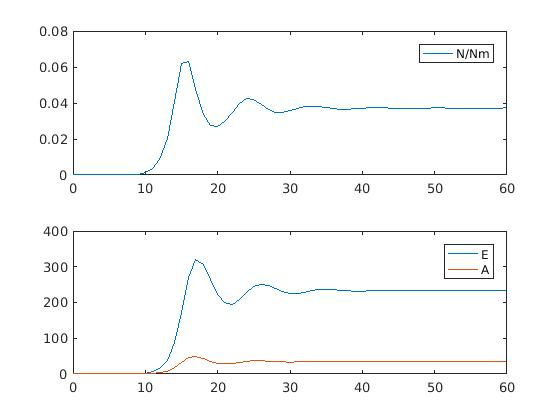
\includegraphics[width=0.7\linewidth]{Figure2.jpg}
    \caption{Cell density, E and A Quantities for the You\_R model}
    \label{q5-R}
  \end{center}
\end{figure}

\begin{figure}[!ht]
  \begin{center}
    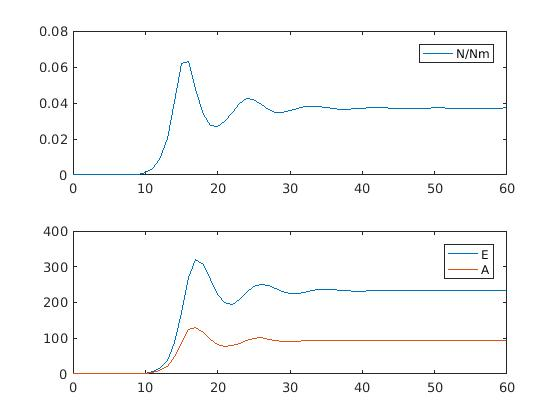
\includegraphics[width=0.7\linewidth]{Figure3.jpg}
    \caption{Cell density, E and A quantities for the You\_I model}
    \label{q5-I}
  \end{center}
\end{figure}

\begin{figure}[!ht]
  \begin{center}
    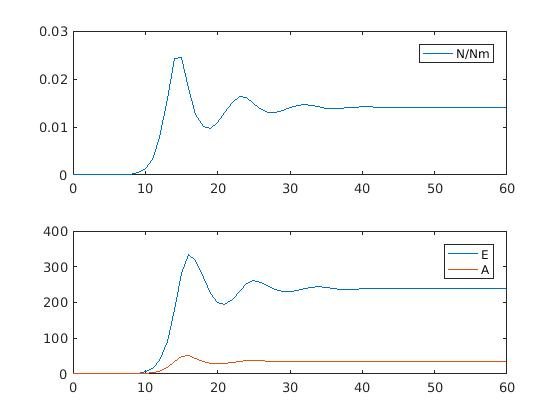
\includegraphics[width=0.7\linewidth]{Figure4.jpg}
    \caption{Cell density, E and A quantities for the You\_RI model}
    \label{q5-RI}
  \end{center}
\end{figure}

In \textsc{Figures}~\ref{q5-R},~\ref{q5-I} and~\ref{q5-RI}, we can see more or less big oscillations, with the system stabilising around the same values (except for N/N$_m$ in \textsc{Figure}~\ref{q5-RI}). Though, we want to control the system \textit{via} an external inducer. In the following questions, we will use it to determine which circuit changes the most in its behaviour regarding the concentration of this inducer.

\section*{Question 6}
In \textsc{Figures}~\ref{q6-N},~\ref{q6-E} and~\ref{q6-A}, we can observe the density of cells, the quantity of E and A regarding different quantities of inducer. Thus, we can see in these figures that, as expected, the behaviour of the You model is not disturbed by the presence of inducer. Though, we can observe that all our new models show a behaviour that depends on the quantity of inducer.

\begin{figure}[!ht]
  \begin{center}
    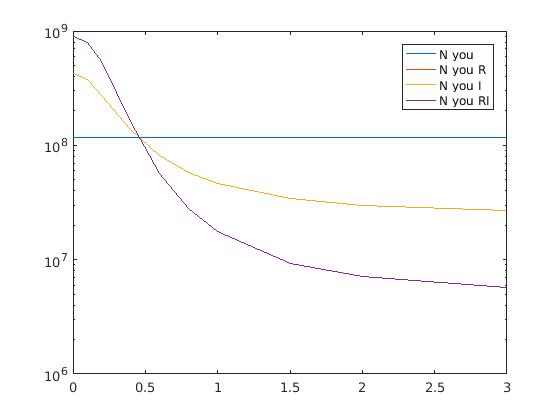
\includegraphics[width=0.7\linewidth]{Figure5.jpg}
    \caption{Cell density for all models}
    \label{q6-N}
  \end{center}
\end{figure}

\begin{figure}[!ht]
  \begin{center}
    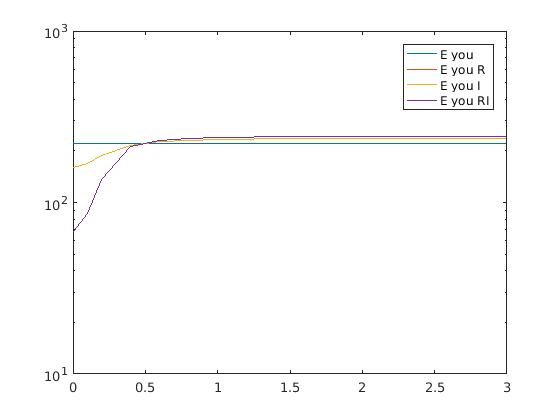
\includegraphics[width=0.7\linewidth]{Figure6.jpg}
    \caption{Concentration of E for all models}
    \label{q6-E}
  \end{center}
\end{figure}

\begin{figure}[!ht]
  \begin{center}
    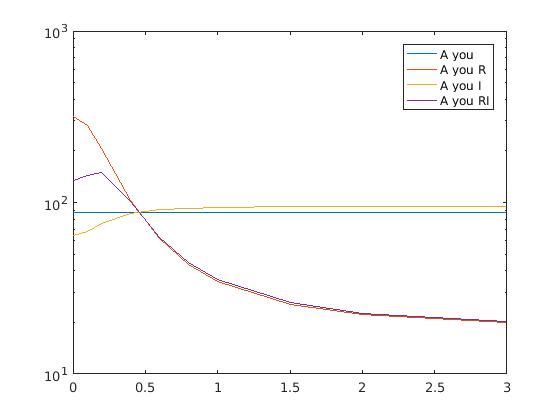
\includegraphics[width=0.7\linewidth]{Figure7.jpg}
    \caption{Concentration of A for all models}
    \label{q6-A}
  \end{center}
\end{figure}
~\\
\newpage
\section*{Question 7}

Using the compute\_msd function, we compute mean squared deviations such as :\\
\begin{center}
\begin{tabular}{|c|c|c||c|c||c|c|}
  \hline
  ~ & R : E & R : A & I : E & I : A & RI : E & RI : A\\
  \hline
  msd & 4.31 & 16.4797 & 4.31004 & 1.72738 & 10.3179 & 10.1225\\
  \hline
\end{tabular}
\end{center}

\section*{Question 8}

Afterward, we compute the variance of the mean squared deviation for each circuit and observed variable, and for each $\theta$ and $\eta$ combination. We get variances such as :\\

\begin{center}
\begin{tabular}{|c|c|c||c|c||c|c|}
  \hline
  ~ & R : E & R : A & I : E & I : A & RI : E & RI : A\\
  \hline
  variance & 2.23808 & 33.0099 & 2.23775 & 0.359261 & 14.0975 & 10.4884\\
  \hline
\end{tabular}
\end{center}
~\\

From this, we can see that the highest variance is the you\_R model one, variable A. We then select this variable for the following computations.\footnote{A copy/paste error in the odes, resulting in the use of wrong parameters, led to a first wrong request of data (you\_RI, variable A). After correcting this mistake, we got a second data set (you\_R, variable A)}

\section*{Question 9}

\begin{figure}[!ht]
  \begin{center}
    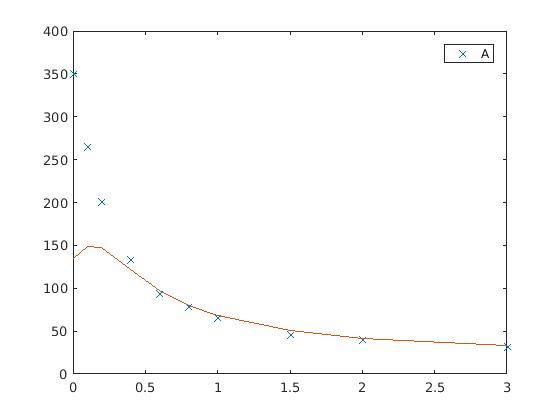
\includegraphics[width=0.7\linewidth]{Figure8.jpg}
    \caption{Concentration of A (you\_R model) given the quantity of inducer}
    \label{q9}
  \end{center}
\end{figure}

In \textsc{Figure}~\ref{q9}, we show the experimental data and the model output after determining the values of $\theta$ and $\eta$ are using cmaes. We can see in that these values are poorly caracterized for low quantities of inducer. Though, for higher quantities, the model output seems to be similar to the experimental data. \\

\section*{Question 10}
As we can see in \textsc{Figure}~\ref{q10}, the highest ratio between inducer presence and absence is showed by the you\_RI circuit. This circuit shows a $\frac{N_{min.~inducer} }{N_{max.~inducer}}$ 8 times higher than the 2 other new circuits. Thus, this is the one we have to use to get a better modulation capability.
\begin{figure}[!ht]
  \begin{center}
    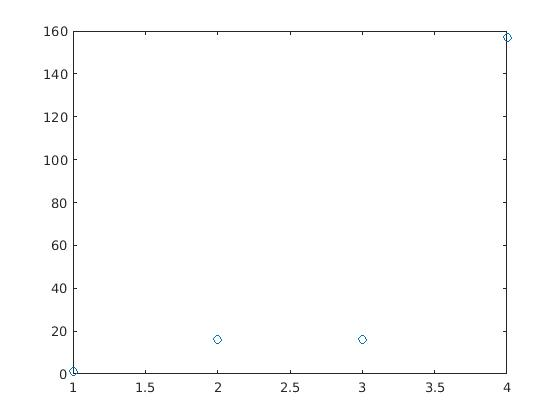
\includegraphics[width=0.7\linewidth]{Figure9.jpg}
    \caption{Plot of the $\frac{N_{min.~inducer} }{N_{max.~inducer}}$ for the You, you\_R, you\_I and you\_RI models}
    \label{q10}
  \end{center}
\end{figure}

\section*{Conclusion}

We can see in \textsc{Figure}~\ref{qC} that we can actually observe a modulation of the cell density using an inducer that we can add to the medium without changing its pH. Thus we can say that our goal has been reached.\\

\begin{figure}[!ht]
  \begin{center}
    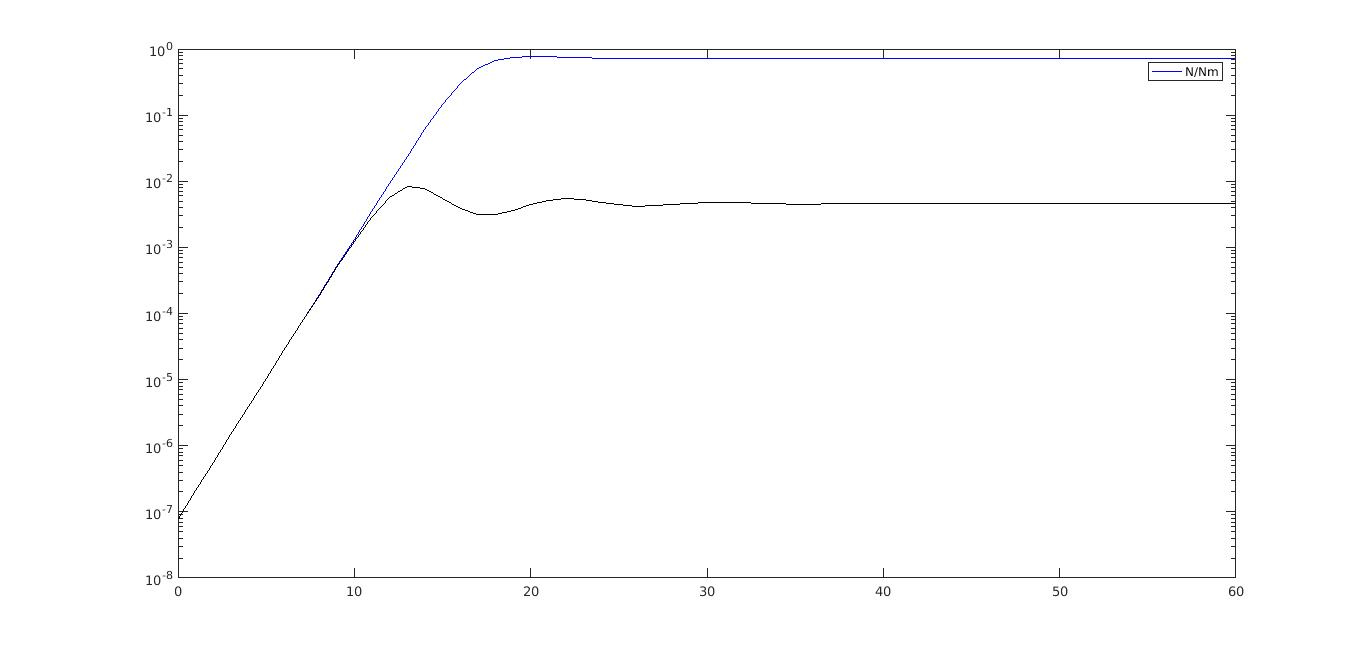
\includegraphics[width=\linewidth]{Figure10.jpg}
    \caption{Plot time behaviour of the cell density with the you\_RI model}
    \label{qC}
  \end{center}
\end{figure}



\end{document}
